\documentclass[12pt]{article}
\usepackage{light}

\newcommand{\spa}{\spadesuit}
\newcommand{\hea}{\heartsuit}
\newcommand{\dia}{\diamondsuit}
\newcommand{\clu}{\clubsuit} 


\hidesolutions
\showsolutions

\begin{document}

\recitation{16}{November 16, 2016}

%%%%%%%%%%%%%%%%%%%%%%%%%%%%%%%%%%%%%%%%%%%%%%%%%%%%%%%%%%%%%%%%%%%%%%%%%%%%%%%

\section{Combinatorial Proof}

A \term{combinatorial proof} is an argument that establishes an
algebraic fact by relying on counting principles.  Many such proofs
follow the same basic outline:
%
\begin{enumerate}

\item Define a set $S$.

\item Show that $\size{S} = n$ by counting one way.

\item Show that $\size{S} = m$ by counting another way.

\item Conclude that $n = m$.

\end{enumerate}

Consider the following theorem:

\begin{theorem*}
\[
\sum_{i=0}^n \binom{k+i}{k} = \binom{k+n+1}{k+1}
\]
\end{theorem*}

We can prove it with a combinatorial approach:

\begin{proof}
We give a combinatorial proof.  Let $S$ be the set of all binary
sequences with exactly $n$ zeroes and $k + 1$ ones.

On the one hand, we know from a previous recitation that the number of
such sequences is equal to $\binom{k + n + 1}{k+1}$.

On the other hand, the number of zeroes $i$ to the left of the rightmost
one ranges from 0 to $n$.  For a fixed value of $i$, there are
$\binom{k + i}{k}$ possible choices for the sequence of bits before the
rightmost one.  If we sum over all possible $i$, we find that
$|S| = \sum_{i = 0}^n \binom{k + i}{k}$.

Equating these two expressions for $\size{S}$ proves the theorem.
\end{proof}
% end insolutions
%}


%%%%%%%%%%%%%%%%%%%%%%%%%%%%%%%%%%%%%%%%%%%%%%%%%%%%%%%%%%%%%%%%%%%%%%%%%%%%%%%

\subsection*{Triangles}
Let $T=\{X_1,\ldots, X_t\}$ be a set whose elements $X_i$ are themselves
sets such that each $X_i$ has size 3 and is $\subseteq \{1,2,\ldots, n\}$.
We call the elements of $T$ ``triangles''. Suppose that for all
``edges'' $E\subseteq \{1,2,\ldots, n\}$ with $|E|=2$ there are exactly
$\lambda$ triangles $X\in T$ with $E\subseteq X$.

For example, if we might have the triangles depicted in the following
diagram, which has $\lambda = 2$, $n = 4$, and $t = 4$:

\begin{center}
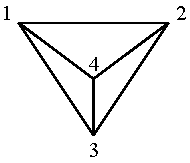
\includegraphics[height=1.5in]{triangles2}
\end{center}

In this example, each edge appears in exactly two of the following triangles:

$$\{1, 2, 3\}, \{1, 2, 4\}, \{1, 3, 4\}, \{2, 3, 4\}$$

Prove
$$ \lambda \cdot \frac{n(n-1)}{2} = 3t$$
by counting the set
$$C= \{ (E,X) : X\in T, E\subseteq X, |E|=2\}$$
in two different ways.

\solution[\vspace{1.5in}]{
We give a combinatorial proof.  Let $C$ be
$\{ (E,X) : X\in T, E\subseteq X, |E|=2\}$.

On the one hand, there are ${n \choose 2}$ sets $E\subseteq \{1,\ldots, n\}$
of size $|E|=2$. For each such $E$ there are exactly $\lambda$
triangles $X\in T$ with $E\subseteq X$. So,
$|C|=\lambda {n \choose 2} = \lambda \cdot \frac{n(n - 1)}{2}$.

On the other hand, there are $t$ triangles. Each triangle has exactly
${3 \choose 2}=3$
subsets $E$ of size 2. So, $|C|=3t$.

Equating these two expressions for $|C|$ proves the theorem.
}

\section{Generating Functions}
The \term{(ordinary) generating function} for a sequence $\seq{a_0, a_1,
a_2, a_3, \dots}$ is the power series:
%
\[
a_0 + a_1 x + a_2 x^2 + a_3 x^3 + \cdots
\]

%%%%%%%%%%%%%%%%%%%%%%%%%%%%%%%%%%%%%%%%%%%%%%%%%%%%%%%%%%%%%%%%%%%%%%%%%%%%%%%

\subsection*{Problem 1}
Find closed-form generating functions for the following sequences.  Do
not concern yourself with issues of convergence.

\begin{enumerate}[(a)]

\item $\seq{2, 3, 5, 0, 0, 0 , 0, \ldots}$

\solution[\vspace{0.25in}]{
\[
2 + 3x + 5x^2
\]
}

\item $\seq{1, 1, 1, 1,1 ,1, 1, \dots}$

\solution[\vspace{0.25in}]{
\[
1 + x + x^2 + x^3 + \ldots = \frac{1}{1 - x}
\]
}

\item $\seq{1, 2, 4, 8, 16, 32, 64, \dots}$

\solution[\vspace{0.25in}]{
\begin{align*}
1 + 2 x + 4 x^2 + 8 x^3 + \ldots
    & = (2x)^0 + (2x)^1 + (2x)^2 + (2x)^3 + \ldots \\
    & = \frac{1}{1 - 2 x}
\end{align*}
}

\item $\seq{1, 0, 1, 0, 1, 0, 1, 0, \dots}$

\solution[\vspace{0.25in}]{
\begin{align*}
1 + x^2 + x^4 + x^6 + \ldots
    & = \frac{1}{1 - x^2}
\end{align*}
}

\item $\seq{0, 0, 0, 1, 1, 1, 1, 1, \dots}$

\solution[\vspace{0.25in}]{
\begin{align*}
x^3 + x^4 + x^5 + x^6 + \ldots
    & = x^3 (1 + x + x^2 + x^3 + \ldots)
    & = \frac{x^3}{1 - x}
\end{align*}
}

\item $\seq{1, 3, 5, 7, 9, 11, \ldots}$

\solution[\vspace{0.25in}]{
\begin{align*}
1 + x + x^2 + x^3 + \ldots & = \frac{1}{1-x} \\
\frac{d}{dx}\ 1 + x + x^2 + x^3 + \ldots & = \frac{d}{dx}\ \frac{1}{1-x} \\
1 + 2 x + 3 x^2 + 4 x^2 + \ldots & = \frac{1}{(1-x)^2} \\
2 + 4 x + 6 x^2 + 8 x^2 + \ldots & = \frac{2}{(1-x)^2} \\
1 + 3 x + 5 x^2 + 7 x^3 + \ldots & = \frac{2}{(1-x)^2} - \frac{1}{1-x} \\
                             & = \frac{1 + x}{(1-x)^2}
\end{align*}
}


\end{enumerate}


%%%%%%%%%%%%%%%%%%%%%%%%%%%%%%%%%%%%%%%%%%%%%%%%%%%%%%%%%%%%%%%%%%%%%%%%%%%%%%%

\newpage

\subsection*{Problem 2}

Suppose that:
%
\begin{align*}
f(x) & = a_0 + a_1 x + a_2 x^2 + a_3 x^3 + a_4 x^4 + \cdots \\
g(x) & = b_0 + b_1 x + b_2 x^2 + b_3 x^3 + b_4 x^4 + \cdots
\end{align*}
%
What sequences do the following functions generate?

\begin{enumerate}[(a)]

\item $f(x) + g(x)$

\solution[\vspace{1in}]{
\[
(a_0 + b_0) + (a_1 + b_1) x + (a_2 + b_2) x^2 + (a_3 + b_3) x^3 + \ldots
\]
}

\item $f(x) \cdot g(x)$

\solution[\vspace{1in}]{
\[
a_0 b_0 + (a_0 b_1 + a_1 b_0) x + (a_0 b_2 + a_1 b_1 + a_2 b_0) x^2 + \ldots
+ \left(\sum_{k=0}^n a_k b_{n-k}\right) x^n + \ldots
\]
}

\item $f(x) / (1 - x)$

\solution{This is a special case of the preceding problem part where:
%
\begin{align*}
g(x) & = \frac{1}{1 - x} \\
     & = 1 + x + x^2 + x^3 + x^4 + \cdots
\end{align*}
%
and so $b_0 = b_1 = b_2 = \ldots = 1$.  In this case, we have:
%
\[
f(x) \cdot g(x) = a_0 + (a_0 + a_1) x + (a_0 + a_1 + a_2) x^2 + \ldots
+ \left(\sum_{k=0}^n a_k \right) x^n + \ldots
\]
%
Thus, $f(x) / (1 - x)$ is the generating function for sums of prefixes
of the sequence generated by $f$.}

\end{enumerate}

%%%%%%%%%%%%%%%%%%%%%%%%%%%%%%%%%%%%%%%%%%%%%%%%%%%%%%%%%%%%%%%%%%%%%%%%%%%%%%%

\newpage

\subsection*{Problem 3}

There is a jar containing $n$ different flavors of candy (and lots of each kind).  I'd like to
pick out a set of $k$ candies.

\begin{enumerate}[(a)]

\item In how many different ways can this be done?

\solution[\vspace{1.25in}]{There is a bijection with sequences
containing $k$ zeroes (representing candies) and $n - 1$ ones
(separating the different varieties).  The number of such sequences
is:
%
\[
\binom{n + k - 1}{k}
\]
}

\item Now let's approach the same problem using generating functions.
Give a closed-form generating function for the sequence $\seq{s_0,
s_1, s_2, s_3, \ldots}$ where $s_k$ is the number of ways to select
$k$ candies when there is only $n = 1$ flavor available.

\solution[\vspace{1.25in}]{
\[
1 + x + x^2 + x^3 + \ldots = \frac{1}{1-x}
\]
}

\item Give a closed-form generating function for the sequence
$\seq{t_0, t_1, t_2, t_3, \ldots}$ where $t_k$ is the number of ways
to select $k$ candies when there are $n = 2$ flavors.

\solution[\vspace{1.25in}]{
\[
(1 + x + x^2 + x^3 + \ldots)^2 = \frac{1}{(1-x)^2}
\]
}

\item Give a closed-form generating function for the sequence
$\seq{u_0, u_1, u_2, u_3, \ldots}$ where $u_k$ is the number of ways
to select $k$ candies when there are $n$ flavors.

\solution[\vspace{1.25in}]{
\[
\frac{1}{(1-x)^n}
\]
}

\end{enumerate}
\end{document}
